\documentclass{article}


% if you need to pass options to natbib, use, e.g.:
%     \PassOptionsToPackage{numbers, compress}{natbib}
% before loading neurips_2023


% ready for submission
\usepackage[preprint]{neurips_2023}
\usepackage{multirow}
\usepackage{tabularx}
\usepackage{tikz}
\usetikzlibrary{matrix,calc}  % <-- load the matrix library
\usepackage{subcaption}  
\usepackage{pgfplots}
\pgfplotsset{compat=1.18}
\usepackage{enumitem}
\usepackage[table,xcdraw]{xcolor}
% to compile a preprint version, e.g., for submission to arXiv, add add the
% [preprint] option:
%     \usepackage[preprint]{neurips_2023}


% to compile a camera-ready version, add the [final] option, e.g.:
%     \usepackage[final]{neurips_2023}
\usepackage{amsmath}
\newcommand{\logits}{\mathbf{z}}

% to avoid loading the natbib package, add option nonatbib:
%    \usepackage[nonatbib]{neurips_2023}

\usepackage{graphicx} 
\usepackage[utf8]{inputenc} % allow utf-8 input
\usepackage[T1]{fontenc}    % use 8-bit T1 fonts
\usepackage{hyperref}       % hyperlinks
\usepackage{url}            % simple URL typesetting
\usepackage{booktabs}       % professional-quality tables
\usepackage{amsfonts}       % blackboard math symbols
\usepackage{nicefrac}       % compact symbols for 1/2, etc.
\usepackage{microtype}      % microtypography
\usepackage{xcolor}         % colors
\newcommand{\todo}[1]{\textcolor{red}{[TODO: #1]}}
\definecolor{darkgreen}{RGB}{0,64,0}



% The \author macro works with any number of authors. There are two co mands
% used to separate the names and addresses of multiple authors: \And and \AND.
%
% Using \And between authors leaves it to LaTeX to determine where to break the
% lines. Using \AND force  a line break at that point. So, if LaTeX put  3 of 4
% authors names on the first line, and the last on the second line, try using
% \AND instead of \And before the third author name.


\author{%
    \textbf{Iwo Godzwon}\textsuperscript{1} \\[0.5em] % Bold author, little space below
    \small Supervisor: Nanne van Noord\textsuperscript{1} \\[1em] % Smaller font for supervisor
    \textsuperscript{1}\small University of Amsterdam, The Netherlands \\
    \small \texttt{iwo.godzwon@student.uva.nl}
}


\begin{document}
\title{Meta-based Concept Bottleneck Models for Interpretable Geolocation}



\maketitle




% \begin{abstract}
% We present Meta-based Concept Bottleneck Models (Meta-CBMs) for interpretable geolocation from StreetView panoramas. Unlike traditional CBMs that require manually curated concept vocabularies, our approach automatically extracts visual concepts from user-generated metadata in GeoGuessr—a geolocation game where players annotate panoramas with descriptive labels. We use Large Language Models to normalize these noisy metadata labels into a structured visual taxonomy (e.g., mapping "RN14" to \texttt{road\_paved}, "Russian storefront" to \texttt{script\_cyrillic}), then train a patch-based CBM that predicts these meta-derived concepts using attention mechanisms. Our experiments show that combining concept predictions with image features achieves 11.86\% lower geolocation error compared to image-only baselines, with median error of 103.4 km and 49.35\% accuracy within 100 km. The meta-derived concepts provide interpretable evidence score maps that highlight spatially meaningful patches, enabling both accurate geolocation and explainable predictions.
% \end{abstract}
\section{Introduction}

GeoGuessr, a popular online game where players guess locations from StreetView panoramas, has attracted millions of players who excel at identifying geographic locations through visual reasoning. What makes expert GeoGuessr players successful is their ability to recognize subtle visual cues: the type of road surface, architectural styles, vegetation patterns, languages, and countless other features that encode geographic information. These players effectively study and apply a discovered set of \textit{metas} like "car meta," "pole shape," or "road paved" that greatly aid in the detection of a downstream location.

This approach differs fundamentally from how machine learning models typically solve geolocation. Deep learning models trained on thousands to millions of images can learn complex patterns directly from pixel data, effectively developing their own internal "metas" that may be highly discriminative but lack human interpretability. For instance, a model might learn to rely on subtle patterns in sky color, specific road texture details, or other low-level features that are difficult for humans to articulate. While these learned features can achieve high accuracy, they are often black-box representations that provide little insight into \textit{why} a location was predicted.

The main motivation in our research is whether models could benefit from human-developed metas, and whether we can make them approach location prediction in a similar way to expert GeoGuessr players, using interpretable concepts rather than opaque internal representations.


[STILL IMPROVE BASED ON REMAINING ]


We introduce \textit{Meta-based Concept Bottleneck Models}, which automatically extract visual concepts from user-generated GeoGuessr metadata and incorporate them into a Concept Bottleneck Model architecture. Our approach normalizes noisy metadata labels into a structured visual concept taxonomy using Large Language Models, then trains a model to predict these human-understandable concepts before making location predictions. The concept predictions are combined with image features for final geolocation, providing both improved accuracy and interpretable evidence score maps that highlight key visual aspects.

Our experiments demonstrate that incorporating human-developed metas significantly improves geolocation performance. Combining concept predictions with image features achieves a 13.5\% mean improvement over image-only baselines on a held-out test set, with median error of 105.3 km. The approach helps on 53.2\% of test samples, providing interpretable evidence score maps that enable explainable predictions. Evaluation on out-of-distribution data reveals an important limitation: performance degrades as expected (mean error 1548.7 km, median 293.7 km), indicating that the model's concept predictions are sensitive to distribution shifts. However, despite this degradation, our approach still maintains its advantage over image-only baselines on OOD data, demonstrating that while human-developed concepts are not immune to distribution shift, they provide a robust foundation that outperforms purely pixel-based representations even when tested on different data distributions.

\section{Related Work}

\subsection{Image Geolocation}
Research in image geolocation has historically progressed from discovering explicit local patterns to training global-scale deep neural networks. 

Before the popularization of deep learning, approaches focused on identifying discriminative visual elements that characterize specific regions. Doersch et al. \cite{10.1145/2830541} showcased this approach with their work "What Makes Paris Look like Paris?", which used discriminative clustering and SVMs to automatically discover interpretable patches, such as distinctive balconies, street signs, or window railings, that distinguish a city.

The field of deep learning allowed scaling towards global classification. Weyand et al. \cite{Weyand_2016} introduced PlaNet, a Convolutional Neural Network (CNN) architecture that framed geolocation as a classification problem by representing the globe as a set of cells. This approach demonstrated that deep models could learn geographic features from pixel data on a large scale, moving away from the explicit feature mining of earlier works.

Current state-of-the-art (SOTA) approaches leverage large-scale pre-training and Vision-Language Models (VLMs) to further refine these representations. StreetCLIP \cite{haas2023learning} adapted the CLIP architecture to the geolocation domain by fine-tuning on StreetView panoramas and location captions, establishing a robust zero-shot baseline. Building on this, PIGEON \cite{haas2024pigeonpredictingimagegeolocations} combines a StreetCLIP-based encoder with a hierarchical geocell classification head and fine-grained offset regression, achieving high accuracy on StreetView benchmarks. Similarly, GeoCLIP \cite{cepeda2023geoclipclipinspiredalignmentlocations} enforces geographic alignment by directly contrasting image embeddings with learned GPS coordinate embeddings, rather than textual descriptions.

Most recently, research has begun to revisit the role of explicit semantic reasoning. NAVIG \cite{zhang2025navignaturallanguageguidedanalysis} introduced an agentic pipeline that employs Vision-Language Models (VLMs), fine-tuned via LoRA on GeoGuessr expert reasoning, to analyze visual clues. To refine its predictions, the system utilizes a suite of external tools, including a retrieved "guidebook" of geolocation tips and a map module. However, this agentic workflow is computationally heavyweight, relying on a complex, multi-stage inference process. Unlike our proposed method, which directly optimizes for a structured taxonomy of human-interpretable concepts within a single forward pass, NAVIG’s reliance on iterative tool use and VLM reasoning makes it less efficient and harder to deploy at scale.

\subsection{Concept Bottleneck Models}

Concept Bottleneck Models \cite{koh2020conceptbottleneckmodels} are a class of interpretable deep learning models that enable explainable predictions by introducing an intermediate layer of human-understandable concepts between input and output. The downstream task predictions are bottlenecked through this middle layer, which represents each image as a set of concepts with their corresponding activations. In the basic CBM framework, training requires concept-level annotations for each image, where each concept must be labeled, making the approach expensive and limiting scalability to new domains.

In recent work, \cite{jia2025interpretablegeolocalizationconceptawareglobal} applied this paradigm to geo-localization, demonstrating that incorporating visual concepts can improve both accuracy and interpretability. Their framework aligns image embeddings with a custom geographical concept set,  derived from knowledge graphs, focusing on attributes such as "climate," "terrain," or broad architectural styles. However, the details of their concept generation pipeline remain unclear, and the unavailability of their implementation poses significant challenges for reproducibility.

Our work builds on this concept-based direction but diverges in two key aspects to address the specific challenges of competitive GeoGuessr. First, rather than relying on general geographic attributes, we focus on player-discovered "metas" (e.g., camera artifacts, specific road markings) that are distinct from standard encyclopedic knowledge. Second, while \cite{jia2025interpretablegeolocalizationconceptawareglobal} utilize a contrastive approach to align global image features, we formulate the problem using MIL. This encourages the model to reason about the geolocation problems, as humans would, enabling interpretability through explicit visual grounding.


\subsection{Multiple Instance Learning for Vision}

Multiple Instance Learning (MIL) is a weakly supervised learning paradigm where training data is organized into sets, or "bags," rather than individual labeled examples \cite{Dietterich1997SolvingTM}. In this formulation, a single class label is assigned to the entire bag, while the labels of the individual instances contained within remain unknown.

Standard MIL approaches typically rely on the assumption that a bag is labeled positive if it contains at least one positive instance, and negative only if all instances are negative \cite{Dietterich1997SolvingTM}. In the context of geolocation, this reflects the expert player's reasoning: a location (bag) is identifiable not because every pixel is distinct, but because a specific subset of patches, such as a unique bollard or license plate, provides the hint on where the location is, whereas the majority of the panorama (e.g., sky, pavement) may be non-informative.

However, traditional MIL methods often assume that instances are Independent and Identically Distributed (i.i.d.), thereby disregarding the correlation among different patches. Although this assumption simplifies the problem, it is often invalid in complex visual tasks where the context and relationship between patches are critical for correct classification. To address this limitation, the TransMIL architecture proposed by Shao et al. integrates the MIL framework with a Transformer-based design to explicitly model the dependencies between instances \cite{shao2021transmiltransformerbasedcorrelated}. This allows the model to aggregate information between different visual cues across the image, rather than treating them in isolation.


\section{Methodology}
We propose a two-stage Meta-based Concept Bottleneck Model for interpretable geolocation from StreetView panoramas. Our approach consists of three main components: (1) data collection and preprocessing, where we extract user-generated metadata from GeoGuessr and normalize it into a structured visual concept taxonomy using Large Language Models; (2) Phase 1 concept classification, where we train a patch-based CBM to predict meta-derived concepts using Multiple Instance Learning; and (3) Phase 2 geolocation, where we combine concept predictions with image features to predict geographic location using a geocell classification approach with fine-grained offset regression. In this section, we describe each component in detail.


\subsubsection{Dataset Construction and Refinement}
We constructed our primary dataset by scraping image-metadata pairs and their associated descriptions from the Learnable Meta platform \cite{LearnableMeta2025}. This collection process yielded a corpus of approximately $43,000$ images associated with $7,289$ unique meta identifier and note pairs.
Upon inspection, the raw dataset exhibited significant label redundancy and inconsistent granularity. The original meta names contained location-specific attributes (e.g., "New York License Plate," "Mexico License Plate"), route identifiers (e.g., "RN14," "Ruta 9"), and country-specific variations that made learning difficult for a computer vision model.


To address this, we implemented a concept generalization strategy using proprietary LLMs. For each unique meta identifier and note pair, the LLM was instructed to generate a standardized, visually meaningful concept label following a hierarchical naming scheme. The generalization process removed location-specific, brand-specific, and route-specific information while preserving visually discriminative attributes. Broad categories (e.g., road, landscape, vegetation, building) were refined into meaningful subtypes (e.g., \texttt{road\_paved}, \texttt{landscape\_hills\_temperate}, \texttt{vegetation\_forest\_boreal}), and text-related concepts were mapped to script families (e.g., \texttt{script\_cyrillic}, \texttt{script\_arabic}). The resulting labels follow a maximum three-part hierarchical structure (category\_subtype\_biome), ensuring consistent granularity across the dataset. This process significantly reduced the number of unique concept labels to 189, while maintaining visual discriminability, creating a more learnable label space for the computer vision model.

We acknowledge that this automated generalization strategy may introduce label noise due to the probabilistic nature of LLMs. While an exhaustive manual verification of all $7,289$ original concepts was infeasible within the scope of this work, we conducted a qualitative manual inspection on a representative subset of the mappings. This analysis confirmed that the unified labels, while subject to semantic imperfections, are sufficiently robust to serve as reliable supervision signals. Consequently, we proceed with this taxonomy as an effective trade-off between semantic precision and the scalability required for large-scale concept learning.


\subsection{Phase 1: Concept Detection}

Phase 1 trains a sparse Concept Bottleneck Model on the extracted metas from StreetView panoramas. The architecture operates on patch tokens extracted from a pre-trained StreetCLIP encoder, which provides rich visual representations while maintaining spatial structure. Each panorama is decomposed into a $24 \times 24$ grid of patches (576 total), where each patch token encodes a local region of the image. This patch-based formulation enables fine-grained interpretability by allowing the model to identify which specific spatial regions contribute to each concept prediction.


\subsubsection{Patch Projection and Mixing}

Given patch tokens $\mathbf{P} \in \mathbb{R}^{B \times 576 \times d_p}$ extracted from the StreetCLIP backbone (where $d_p = 1024$), we first project them into a concept-aligned feature space of dimension $d_c$:

\begin{equation}
\mathbf{X} = \text{Project}(\mathbf{P}) \in \mathbb{R}^{B \times 576 \times d_c}
\end{equation}

The projection function $\text{Project}(\cdot)$ is implemented as a learnable linear layer. This design was chosen to serve as a lightweight adaptation layer between the general-purpose visual features of StreetCLIP and our specific "meta" concept space, while minimizing the risk of overfitting associated with deeper non-linear adaptors.

To preserve the spatial structure inherent in panoramic imagery, we add learnable 2D positional encodings to the projected tokens $\mathbf{X}$. Subsequently, a Transformer-based patch mixer contextualizes each patch with standard \textit{Self-Attention}.

\subsubsection{Concept Query Formulation}\label{sec:concept-queries}

We define a set of learnable concept queries $\mathbf{Q} \in \mathbb{R}^{K \times d_c}$, where $K$ is the number of concept classes and $d_c = 256$ is the concept embedding dimension. Each row $\mathbf{q}_k \in \mathbb{R}^{d_c}$ represents a learnable prototype vector that encodes the visual signature of concept $k$. These queries act as semantic anchors that probe the projected patch features $\mathbf{X} \in \mathbb{R}^{B \times P \times d_c}$ (where $B$ is the batch size and $P$ is the number of patches) to compute evidence scores indicating the presence of each concept.

The evidence score for concept $k$ at patch $p$ is computed via a dot product:
\begin{equation}
s_{k,p} = \mathbf{q}_k^T \mathbf{x}_p + b_k
\end{equation}
where $\mathbf{x}_p \in \mathbb{R}^{d_c}$ is the projected feature vector for patch $p$ (after patch mixing), and $b_k \in \mathbb{R}$ is a learnable bias term. This formulation allows each concept query to independently assess the relevance of spatial patches, enabling the model to identify localized visual evidence.

\textbf{Dimensionality bottleneck.} We explicitly constrain the concept dimension to $d_c = 256$, which is significantly smaller than the pre-trained StreetCLIP patch dimension ($d = 1024$). This dimensionality reduction serves as an information bottleneck, forcing the model to distill only the most discriminative visual patterns and filter out redundant correlations present in the high-dimensional space.

\textbf{Initialization strategy.} While the architecture supports initialization from pre-trained text embeddings, we initialize the queries via Xavier initialization. This design choice differentiates our concept representations from those of the StreetCLIP text encoder. By avoiding rigid text-based priors, we allow the queries to adapt freely to the specific metas discovered by GeoGuessr players, which often are not aligned with the pretraining of StreetCLIP.
\subsubsection{Multiple Instance Learning with Top-K Pooling}

To predict concepts from the mixed patch representations, we formulate the problem using Multiple Instance Learning (MIL), where each panorama is treated as a "bag" of patches, and the concept label applies to the entire bag. This formulation naturally aligns with how expert GeoGuessr players reason: a location is identifiable not because every patch is distinctive, but because a small subset of patches (e.g., a unique road sign or architectural detail) provides the critical evidence.

For each concept $k$, we compute patch-level evidence scores using the learned concept queries $\mathbf{q}_k \in \mathbb{R}^{d_c}$:

\begin{equation}
s_{b,k,p} = \mathbf{q}_k^T \mathbf{x}_{b,p} + b_k
\end{equation}

where $\mathbf{x}_{b,p}$ is the mixed representation of patch $p$ in batch sample $b$, and $b_k$ is a learnable bias term. Rather than aggregating over all 576 patches (which would dilute the signal from discriminative regions), we employ a \textit{hard top-$K$ selection} strategy: for each concept, we identify the $K$ patches with the highest evidence scores (typically $K=6$), then aggregate them using a temperature-scaled LogSumExp pooling:

\begin{equation}
\logits_{b,k} = \tau \cdot \log \sum_{p \in \text{topK}(s_{b,k,:})} \exp(s_{b,k,p} / \tau)
\end{equation}

where $\tau$ is a temperature hyperparameter (typically $\tau = 0.25$) that controls the sharpness of the aggregation. The LogSumExp function provides a smooth approximation of the maximum operation, allowing gradients to flow through all top-$K$ patches while still emphasizing the most discriminative evidence. Low temperatures encourage the model to focus sharply on the most discriminative patches, while higher temperatures allow softer attention over multiple regions. Finally, we enable per-concept adaptive temperature, where each concept learns its own $\tau_k$ during training, allowing localized concepts (e.g., "license plate") to use lower temperatures than scene-level concepts (e.g., "landscape\_mountains").

\textbf{Training regularization.} During training, we employ Selective Top-K Instance Masking (STKIM) \cite{STKIM}. This technique randomly masks the patches with the highest evidence scores with probability $p_{\text{mask}}$, preventing the model from relying exclusively on a single dominant patch to make a prediction. By temporarily removing the most obvious visual cues (such as distinct sky patterns or simple artifacts), the mechanism forces the network to identify alternative supporting evidence in other regions. This encourages the model to learn a more robust set of features rather than overfitting to convenient shortcuts.


\subsubsection{Alternative Architecture: Cross-Attention Concept Head}

As an alternative to the dot-product scoring approach, we explore a cross-attention architecture where learned concept tokens serve as queries that attend to patch representations as keys and values. This design allows concepts to learn more expressive query patterns through learned $Q$, $K$, and $V$ projections, potentially capturing complex relationships between patches that simple dot products cannot express.

\subsubsection{Training Objective}

Phase 1 is trained using a standard cross-entropy loss with label smoothing ($\epsilon = 0.1$) to prevent overconfidence:

\begin{equation}
\mathcal{L}_{\text{CE}} = -\sum_{b=1}^{B} \log \frac{\exp(\logits_{b,y_b} + \epsilon/K)}{\sum_{k=1}^{K} \exp(\logits_{b,k})}
\end{equation}

where $y_b$ is the ground-truth concept label for sample $b$, and $K$ is the total number of concepts. To address class imbalance in the concept distribution, we weight the loss by inverse frequency, ensuring that rare but discriminative concepts receive sufficient learning signal. The model is trained for 80 epochs with early stopping based on validation accuracy, using the AdamW optimizer with a learning rate of $7 \times 10^{-5}$ and a 5-epoch warmup period.

\subsection{Phase 2: Joint Training for Geolocation}

Phase 2 combines the concept predictions from Phase 1 with image features to predict geographic locations. We frame geolocation as a two-stage problem: (1) coarse geocell classification to identify the approximate region, and (2) fine-grained offset regression within the predicted geocell to obtain precise coordinates. This hierarchical approach, inspired by PIGEON \cite{haas2024pigeonpredictingimagegeolocations}, enables the model to learn both global geographic patterns and local refinements.

\subsubsection{Concept Embedding Adaptation}

The Phase 1 model outputs concept logits $\mathbf{z} \in \mathbb{R}^{B \times K}$, where each element $z_{b,k}$ represents the evidence score for concept $k$ in sample $b$. To integrate these logits into the geolocation head, we employ a \textit{Concept Embedding Adapter} that converts discrete concept predictions into a continuous embedding space.

The adapter first applies a temperature-scaled softmax to the logits:

\begin{equation}
p_{b,k} = \frac{\exp(z_{b,k} / \tau)}{\sum_{j=1}^{K} \exp(z_{b,j} / \tau)}
\end{equation}

where $\tau$ is a temperature hyperparameter (typically $\tau = 2.5$) that controls the sharpness of the distribution. Higher temperatures produce softer distributions, allowing multiple concepts to contribute to the embedding. The concept embedding is then computed as a weighted combination of learnable concept vectors:

\begin{equation}
\mathbf{c}_b = \sum_{k=1}^{K} p_{b,k} \cdot \mathbf{e}_k
\end{equation}

where $\mathbf{E} \in \mathbb{R}^{K \times d_c}$ is a learnable concept vector bank, and $\mathbf{e}_k$ is the $k$-th row representing concept $k$'s embedding. This formulation allows the model to leverage the full distribution of concept predictions rather than only the top-1 concept, capturing nuanced relationships between multiple visual cues.

\subsubsection{Geocell Formulation}

We partition the globe into a set of semantic geocells using K-means clustering on the training set coordinates, following the approach of PIGEON \cite{haas2024pigeonpredictingimagegeolocations}. Training coordinates are first converted from latitude/longitude to 3D Cartesian coordinates $(x, y, z)$ on the unit sphere:

\begin{align}
x &= \cos(\text{lat}) \cos(\text{lng}) \\
y &= \cos(\text{lat}) \sin(\text{lng}) \\
z &= \sin(\text{lat})
\end{align}

K-means clustering (typically with $K=1000$ clusters) is applied to these 3D coordinates to obtain geocell centers $\mathbf{C} \in \mathbb{R}^{K \times 3}$. Each training sample is assigned to its nearest geocell center, and a 3D offset vector $\boldsymbol{\delta} \in \mathbb{R}^3$ is computed as the difference between the sample's 3D coordinate and its assigned geocell center.

This formulation decomposes geolocation into two subproblems: (1) predicting which geocell $\hat{c}$ the image belongs to (classification), and (2) predicting the fine-grained offset $\hat{\boldsymbol{\delta}}$ within that geocell (regression). The final predicted location is recovered as:

\begin{equation}
\hat{\mathbf{xyz}} = \mathbf{C}[\hat{c}] + \hat{\boldsymbol{\delta}}
\end{equation}

which is then converted back to latitude/longitude coordinates. This hierarchical approach enables the model to learn both coarse geographic patterns (e.g., continent-level distinctions) and fine-grained localizations (e.g., city-level precision).

\subsubsection{Dual-Pathway Architecture with Late Fusion}

We design a dual-pathway architecture that processes image and concept features independently before fusing their predictions. This design ensures both pathways receive direct supervision and learn complementary representations.

\textbf{Image pathway.} The image pathway operates on pooled embeddings $\mathbf{h}_{\text{img}} \in \mathbb{R}^{B \times d_p}$ extracted from the StreetCLIP encoder (typically $d_p = 768$). These embeddings are projected to a shared hidden dimension $d_h$ (typically $d_h = 512$) and passed through an adapter network:

\begin{equation}
\mathbf{h}_{\text{img}}' = \text{Adapter}_{\text{img}}(\text{Proj}_{\text{img}}(\mathbf{h}_{\text{img}})) \in \mathbb{R}^{B \times d_h}
\end{equation}

The adapter consists of LayerNorm, linear projection, GELU activation, and dropout. The adapted features are then passed through separate prediction heads for geocell classification and offset regression:

\begin{align}
\mathbf{z}_{\text{img}}^{\text{cell}} &= \text{Head}_{\text{img}}^{\text{cell}}(\mathbf{h}_{\text{img}}') \in \mathbb{R}^{B \times K} \\
\boldsymbol{\delta}_{\text{img}} &= \text{Head}_{\text{img}}^{\text{offset}}(\mathbf{h}_{\text{img}}') \in \mathbb{R}^{B \times 3}
\end{align}

\textbf{Concept pathway.} The concept pathway operates on the concept embeddings $\mathbf{c}_b \in \mathbb{R}^{B \times d_c}$ produced by the Concept Embedding Adapter. These embeddings are projected to the same hidden dimension and passed through a similar adapter:

\begin{equation}
\mathbf{h}_{\text{concept}}' = \text{Adapter}_{\text{concept}}(\text{Proj}_{\text{concept}}(\mathbf{c}_b)) \in \mathbb{R}^{B \times d_h}
\end{equation}

Separate prediction heads produce concept-based geocell and offset predictions:

\begin{align}
\mathbf{z}_{\text{concept}}^{\text{cell}} &= \text{Head}_{\text{concept}}^{\text{cell}}(\mathbf{h}_{\text{concept}}') \in \mathbb{R}^{B \times K} \\
\boldsymbol{\delta}_{\text{concept}} &= \text{Head}_{\text{concept}}^{\text{offset}}(\mathbf{h}_{\text{concept}}') \in \mathbb{R}^{B \times 3}
\end{align}

\textbf{Gated late fusion.} The two pathways are fused at the logit level using an image-controlled gate mechanism. The gate $\mathbf{g} \in \mathbb{R}^{B \times 1}$ is computed from the image pathway features, allowing the image to determine when to trust concept predictions:

\begin{equation}
\mathbf{g} = \sigma(\text{GateNetwork}(\mathbf{h}_{\text{img}}')) \in [0, 1]^B
\end{equation}

where $\sigma$ is the sigmoid function. The gate is initialized with a negative bias (typically $-4.0$) so that $\mathbf{g} \approx 0$ at the start of training, making the model mathematically identical to an image-only baseline at epoch 0. This initialization ensures the concepts will be used only if their addition helps with the geolocation.

The final predictions are computed as:

\begin{align}
\mathbf{z}^{\text{cell}} &= \mathbf{z}_{\text{img}}^{\text{cell}} + \mathbf{g} \odot \mathbf{z}_{\text{concept}}^{\text{cell}} \\
\boldsymbol{\delta} &= \boldsymbol{\delta}_{\text{img}} + \mathbf{g} \odot \boldsymbol{\delta}_{\text{concept}}
\end{align}

where $\odot$ denotes element-wise multiplication (broadcasted appropriately). This late fusion at the logit level ensures both pathways receive direct gradients through their respective prediction heads, unlike feature-level fusion where one pathway can be ignored.

\subsubsection{Training Objective}

Phase 2 is trained with a multi-task loss combining geocell classification and offset regression. The geocell loss is standard cross-entropy:

\begin{equation}
\mathcal{L}_{\text{cell}} = -\frac{1}{B} \sum_{b=1}^{B} \log \frac{\exp(z_{b,y_b}^{\text{cell}})}{\sum_{k=1}^{K} \exp(z_{b,k}^{\text{cell}})}
\end{equation}

where $y_b$ is the ground-truth geocell label for sample $b$. The offset loss is mean squared error in 3D Cartesian space:

\begin{equation}
\mathcal{L}_{\text{offset}} = \frac{1}{B} \sum_{b=1}^{B} \|\boldsymbol{\delta}_b - \boldsymbol{\delta}_b^*\|_2^2
\end{equation}

where $\boldsymbol{\delta}_b^*$ is the ground-truth offset. The offset loss is scaled by a factor of 1000 to match the magnitude of the classification loss, ensuring both terms contribute meaningfully to the gradient.

The total loss is:

\begin{equation}
\mathcal{L}_{\text{total}} = \lambda_{\text{cell}} \mathcal{L}_{\text{cell}} + \lambda_{\text{offset}} \cdot 1000 \cdot \mathcal{L}_{\text{offset}}
\end{equation}

where $\lambda_{\text{cell}}$ and $\lambda_{\text{offset}}$ are loss weights. 

% Optionally, we include an orthogonality regularizer that encourages the image and concept pathway features to be complementary rather than redundant:

% \begin{equation}
% \mathcal{L}_{\text{ortho}} = \frac{1}{B} \sum_{b=1}^{B} \left(\frac{\mathbf{h}_{\text{img},b}' \cdot \mathbf{h}_{\text{concept},b}'}{\|\mathbf{h}_{\text{img},b}'\|_2 \|\mathbf{h}_{\text{concept},b}'\|_2}\right)^2
% \end{equation}

% This regularizer penalizes high cosine similarity between the two pathways, encouraging them to capture different aspects of geographic information.

During joint training, both the Phase 1 concept model and the geolocation head are updated end-to-end. To maintain stability while still allowing refinement of the concept detector, we use separate learning rates: a lower learning rate for Phase 1 (e.g., $1\times 10^{-5}$) and a higher learning rate for Phase 2 (e.g., $1\times 10^{-4}$). Optimization is performed with AdamW and a cosine annealing learning-rate schedule. We train for up to 100 epochs and apply early stopping with patience 10 based on the validation \emph{median} geolocation error (km).

\section{Results}

\subsection{Implementation Details}

We initialize our model using the pre-trained StreetCLIP encoder \cite{haas2023learning}, which provides robust visual representations for StreetView panoramas. All images are resized to $336 \times 336$ pixels and divided into a $24 \times 24$ grid of patches (576 total patches) using a patch size of 14 pixels. We extract both pooled embeddings ($d_p = 768$) and patch tokens ($d_{patch} = 1024$) from the StreetCLIP backbone, which remain frozen throughout training for computational efficiency.

Our dataset consists of 33,852 training samples, 4,226 validation samples, and 4,265 test samples. For geocell classification, we partition the training set coordinates into $M=1000$ semantic geocells using K-means clustering in 3D Cartesian space.

\subsection{Phase 1: Concept Classification}

We train the Phase 1 concept detector using AdamW optimization with a learning rate of $5 \times 10^{-5}$ for our proposed Top-K MIL model and $7 \times 10^{-5}$ for the text-initialized variant. We use a weight decay of 0.05 and an 8-epoch warmup period (5 epochs for text-init). The models are trained for up to 100 epochs with early stopping based on validation accuracy. We employ cross-entropy loss with label smoothing ($\epsilon = 0.1$) and inverse frequency class weighting to handle concept imbalance.

Our proposed model uses a simple linear projection from StreetCLIP patch features ($d=1024$) to concept space ($d_c=256$), with learnable concept queries initialized via Xavier initialization. This architecture achieves 39.68\% Top-1 accuracy and 69.76\% Top-5 accuracy on the test set (4,229 samples). While we explored architectural variants that achieve marginally higher classification accuracy, we selected this configuration because it produces the \textbf{most interpretable evidence score maps}, highlighting the correct regions in the panoramas most reliably (Fig \ref{fig:attnmaps1}).

To validate our design choice, we evaluated several alternative architectures, summarized in Table \ref{tab:phase1_ablation}:

\begin{table}[h]
\centering
\caption{Phase 1 concept classification performance on test set. All models use Top-K LogSumExp pooling ($K=6$, $\tau=0.25$) and standard Self-Attention.}
\label{tab:phase1_ablation}
\begin{tabular}{lccc}
\toprule
\textbf{Model Variant} & \textbf{Acc@1} & \textbf{Acc@5} & \textbf{CE Loss} \\
\midrule
\textbf{Top-K MIL (Simple 256-dim)} & 39.68\% & 69.76\% & 3.16 \\
\textbf{Text-Init (StreetCLIP Priors)} & 41.90\% & 72.90\% & 3.04 \\
\textbf{Cross-Attention Head} & 34.36\% & 62.26\% & 3.34 \\
\bottomrule
\end{tabular}
\end{table}

The text-initialized variant initializes concept queries from StreetCLIP's text encoder embeddings, providing strong semantic priors from the vision-language model. This initialization helps the model converge to a higher accuracy (41.90\% Top-1), as the queries start in a semantically meaningful space aligned with the visual backbone. However, despite the quantitative improvement, visual inspection of the evidence score maps revealed that the text-initialized model frequently relied on non-semantic background features (Fig \ref{fig:attnmaps1}). We observed that this model often focused on uninterpretable regions, such as specific patches of the sky rather than the distinct objects associated with the concept labels. 

The cross-attention architecture replaces the dot-product scoring with a learned cross-attention mechanism, where concept tokens serve as queries that attend to patch representations. This design allows for more expressive query patterns but underperforms the simpler dot-product approach, achieving only 34.36\% Top-1 accuracy. We attribute this to the increased model complexity and the difficulty of learning effective cross-attention patterns from scratch, especially given the limited training data and the need for interpretable, localized evidence scores. Furthermore, the evidence score maps support the poor learning, as we can observe that the evidence score visualization is seemingly a random blur of patches (Fig \ref{fig:attnmaps1}).

\begin{figure}[h]
\centering
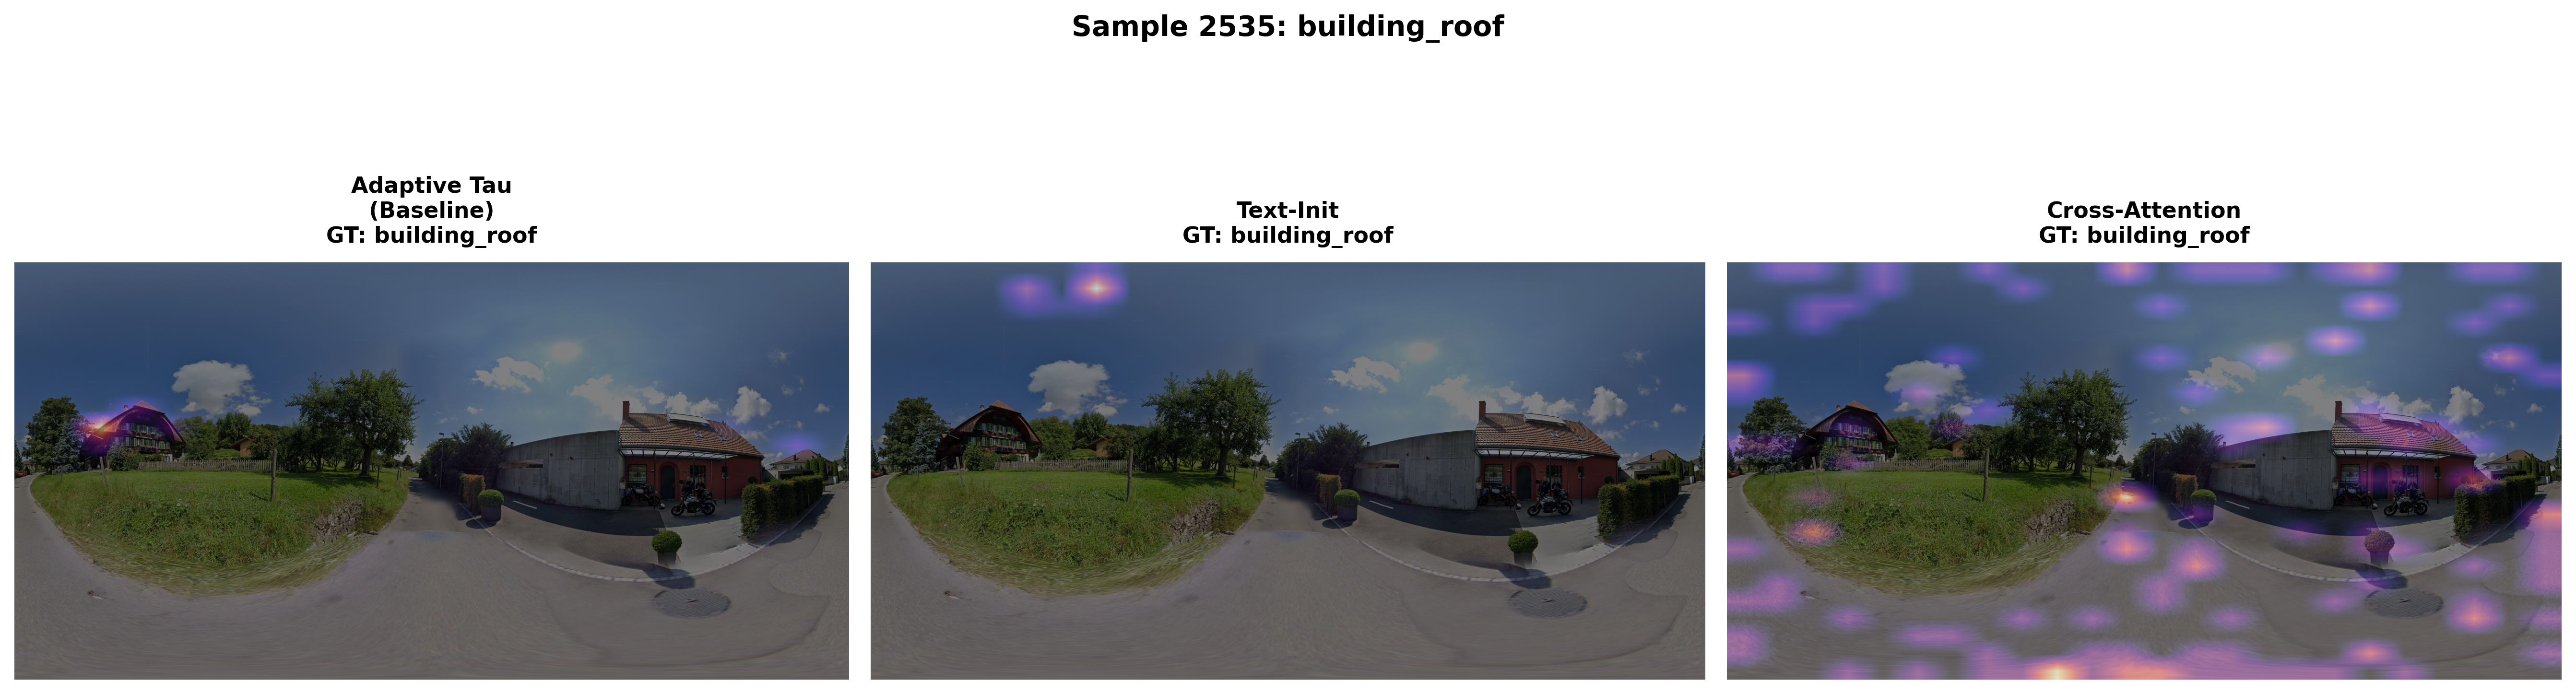
\includegraphics[width=\textwidth]{images/attention_map_comp.png}
\caption{Comparison of evidence score maps across different model architectures for sample 2535. The visualization demonstrates how different architectural choices produce varying evidence score patterns for the same input image and concept. Our proposed Top-K MIL model (left) correctly highlights the building roof depicted in the panorama, while the remaining two images struggle with this task.}
\label{fig:attnmaps1}
\end{figure}

\subsubsection{Phase 2: Geolocation}

We evaluate the same two model variants in the geolocation setting to analyze how differences in the Phase~1 concept detector architectures affect downstream performance. Each variant reuses its corresponding Phase~1 concept detection backbone and is jointly trained with a geolocation head using late fusion with gated concept integration. Quantitative results are reported in Table~\ref{tab:phase2_geolocation}.

Both models achieve competitive performance across all metrics, with relatively small differences between them. The text-initialized variant attains higher concept classification accuracy (42.2\% vs.\ 40.8\% top-1, 73.8\% vs.\ 70.5\% top-5) and marginal improvements in geocell accuracy, median error, and Acc@100km. In contrast, the Top-K MIL model achieves a slightly lower mean geolocation error (745.2~km vs.\ 764.8~km), indicating improved robustness in more challenging cases.

The improved concept accuracy of the text-initialized model can be attributed to the semantic priors provided by StreetCLIP text embeddings, which facilitate concept recognition during joint training. However, these priors can also introduce sharper failure modes when incorrect concepts are activated, contributing to the higher mean error. This behavior is reflected in the gating statistics: the text-initialized model relies more conservatively on concepts (mean gate $0.42 \pm 0.09$), whereas the Top-K MIL model integrates concept information more strongly (mean gate $0.60 \pm 0.13$).

Although the text-initialized variant achieves slightly better performance on several typical-case metrics, the overall performance gap between the two approaches remains modest. Given this closeness, we select the Top-K MIL architecture as our final model based primarily on qualitative considerations aligned with our objectives. In particular, the Top-K MIL model produces substantially more interpretable evidence score maps with clearer spatial localization, as demonstrated in Phase~1 (Fig.~\ref{fig:attnmaps1}). This improved interpretability, combined with its lower mean error, makes the Top-K MIL architecture better suited to our goal of building robust and explainable concept bottleneck models, even in the absence of a strong quantitative advantage.


\subsubsection{In-Distribution Evaluation}

We evaluate three model variants on the held-out test set: (1) \textbf{Image + Concepts} (full model with late fusion), (2) \textbf{Concepts Only} (concept pathway only), and (3) \textbf{Image Only} (image pathway only, our baseline using StreetCLIP). Results are summarized in Table \ref{tab:geolocation_results}.

\begin{table}[h]
\centering
\caption{Geolocation performance on held-out test set (4,265 samples). All distances in kilometers.}
\label{tab:geolocation_results}
\begin{tabular}{lccc}
\toprule
\textbf{Metric} & \textbf{Image + Concepts} & \textbf{Image Only} & \textbf{Concepts Only} \\
\midrule
Mean Error & \textbf{745.2} & 861.4 & 1134.9 \\
Median Error & \textbf{105.3} & 126.9 & 180.6 \\
Acc@10km & \textbf{3.59}\% & 3.24\% & 3.33\% \\
Acc@100km & \textbf{48.9\%} & 46.0\% & 39.7\% \\
Acc@1000km & \textbf{87.8\%} & 85.9\% & 81.3\% \\
Acc@2500km & \textbf{93.9\%} & 93.1\% & 90.4\% \\
\bottomrule
\end{tabular}
\end{table}

Our full model (Image + Concepts) achieves a median error of 105.3 km, representing a \textbf{17.0\%} improvement over the image-only StreetCLIP baseline (126.9 km) and a \textbf{13.5\%} reduction in mean error (745.2 km vs. 861.4 km). The fusion approach improves accuracy at all distance thresholds, with the most significant gains at the 100km threshold (48.9\% vs. 46.0\%) and 1000km threshold (87.8\% vs. 85.9\%). An example of such improvement can be seen in Fig \ref{fig:success_case_study}.

\begin{figure}[h]
\centering
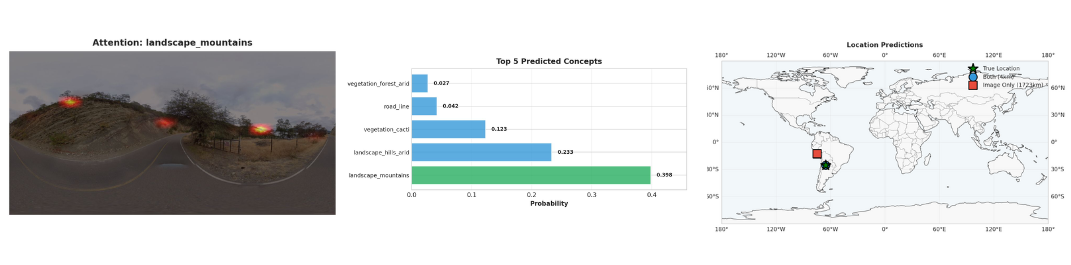
\includegraphics[width=\textwidth]{images/success2.png}
\caption{Example demonstrating how concept predictions improve geolocation accuracy. \textbf{Left:} The model correctly identifies \texttt{landscape\_mountains} as the primary concept (probability 0.398), with evidence score heatmaps highlighting the mountainous terrain in the panorama. The top-5 concept predictions (\texttt{landscape\_mountains}, \texttt{landscape\_hills\_arid}, \texttt{vegetation\_cacti}, etc.) are consistent with the arid, mountainous landscape. \textbf{Right:} Location predictions on a world map. The combined model (Image + Concepts) achieves near-perfect accuracy with only 4 km error, correctly predicting the location. In contrast, the image-only baseline predicts a location 1,723 km away, demonstrating that the \texttt{landscape\_mountains} concept provides critical geographic information that pixel-level features alone fail to capture. This example illustrates how human-interpretable concepts enable both accurate geolocation and explainable predictions.}
\label{fig:success_case_study}
\end{figure}
Notably, the Concepts Only model achieves reasonable geolocation performance despite operating solely on high-level semantic information, with a median error of 180.6 km and 81.3\% accuracy within 1000 km. This demonstrates that human-discovered metas encode substantial geographic signal, though they are insufficient for precise localization without complementary pixel-level features.


\newpage




\subsubsection{Out-of-Distribution Evaluation}

To assess the robustness of our approach to distribution shift, we evaluate both the full model (Image + Concepts) and the image-only StreetCLIP baseline on a out-of-distribution dataset: 5,478 images of random StreetView data \cite{FrenGorGeoGuessrLocations}. The challenge can come from the fact that these images may not exhibit any of the collected metas. This experiment aims to test whether our concept base is large enough to handle any location presented. The results are presented in Table \ref{tab:ood_results}.

\begin{table}[h]
\centering
\caption{Out-of-distribution evaluation on GeoGuessr gameplay data (5,478 samples).}
\label{tab:ood_results}
\begin{tabular}{lcc}
\toprule
\textbf{Metric} & \textbf{Image + Concepts} & \textbf{Image Only} \\
\midrule
Mean Error (km) & \textbf{1548.7} & 1736.5 \\
Median Error (km) & \textbf{293.7} & 344.8 \\
Acc@100km & \textbf{26.2\%} & 24.6\% \\
Acc@1000km & \textbf{75.5\%} & 72.7\% \\
Acc@2500km & \textbf{86.8\%} & 85.5\% \\
Country Accuracy & \textbf{51.1\%} & 49.1\% \\
Continent Accuracy & \textbf{86.1\%} & 84.3\% \\
\bottomrule
\end{tabular}
\end{table}

As expected, performance degrades significantly on OOD data compared to the in-distribution test set. The full model's median error increases from 105.3 km (in-distribution) to 293.7 km (OOD), reflecting the challenge of generalizing to unseen geographic regions. However, \textbf{our concept-based approach maintains its advantage over the image-only StreetCLIP baseline even under distribution shift}: the full model achieves 14.8\% lower median error (293.7 km vs. 344.8 km) on OOD data.
This finding is particularly significant because it demonstrates that human-developed concepts, while not immune to distribution shift, provide a more robust foundation than purely pixel-based representations. The concept pathway appears to capture generalizable semantic patterns (e.g., climate indicators, architectural styles, road infrastructure) that transfer better across different geographic distributions than low-level visual features.

\begin{figure}[h]
\centering
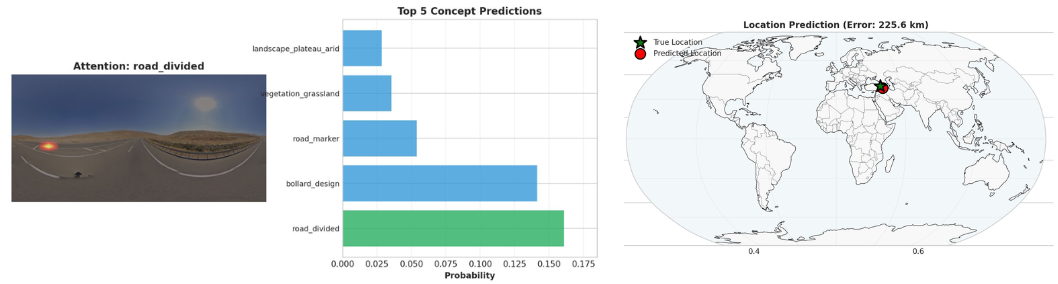
\includegraphics[width=0.9\textwidth]{images/location.png}
\caption{Out-of-distribution example from GeoGuessr gameplay data demonstrating robust concept detection and country-level accuracy. The model correctly identifies \texttt{road\_divided} as the primary concept (probability 0.165) with spatially accurate evidence scores: the heatmap highlights the opposite lane of the divided highway, demonstrating that the model understands the visual structure of divided roads rather than relying on spurious correlations. The evidence score map correctly localizes to the road infrastructure that defines the concept, enabling interpretable reasoning. Despite the distribution shift from training data, the Image + Concepts model achieves country-level accuracy (225.6 km error), correctly localizing to the Turkey region.}
\label{fig:ood_success_case}
\end{figure}

\subsection{Qualitative Analysis: Evidence Score Maps}

We observe substantial variation in activation behavior across concepts, reflecting differences in visual scale, spatial extent, and distinctiveness. Small concepts such as \textit{chevron} exhibit consistently low activation scores, with distributions concentrated near zero. This behavior is also reflected in the corresponding per-concept evidence visualizations, where activations are seemingly random (Fig \ref{fig:chevron_evidence}). A likely contributing factor is the small physical size of chevrons: at the StreetCLIP input resolution of $336 \times 336$ pixels, such thin structures are difficult to resolve reliably. In addition, \textit{chevron} is relatively underrepresented in the training data, with only 123 samples.

\begin{figure}[t]
    \centering
    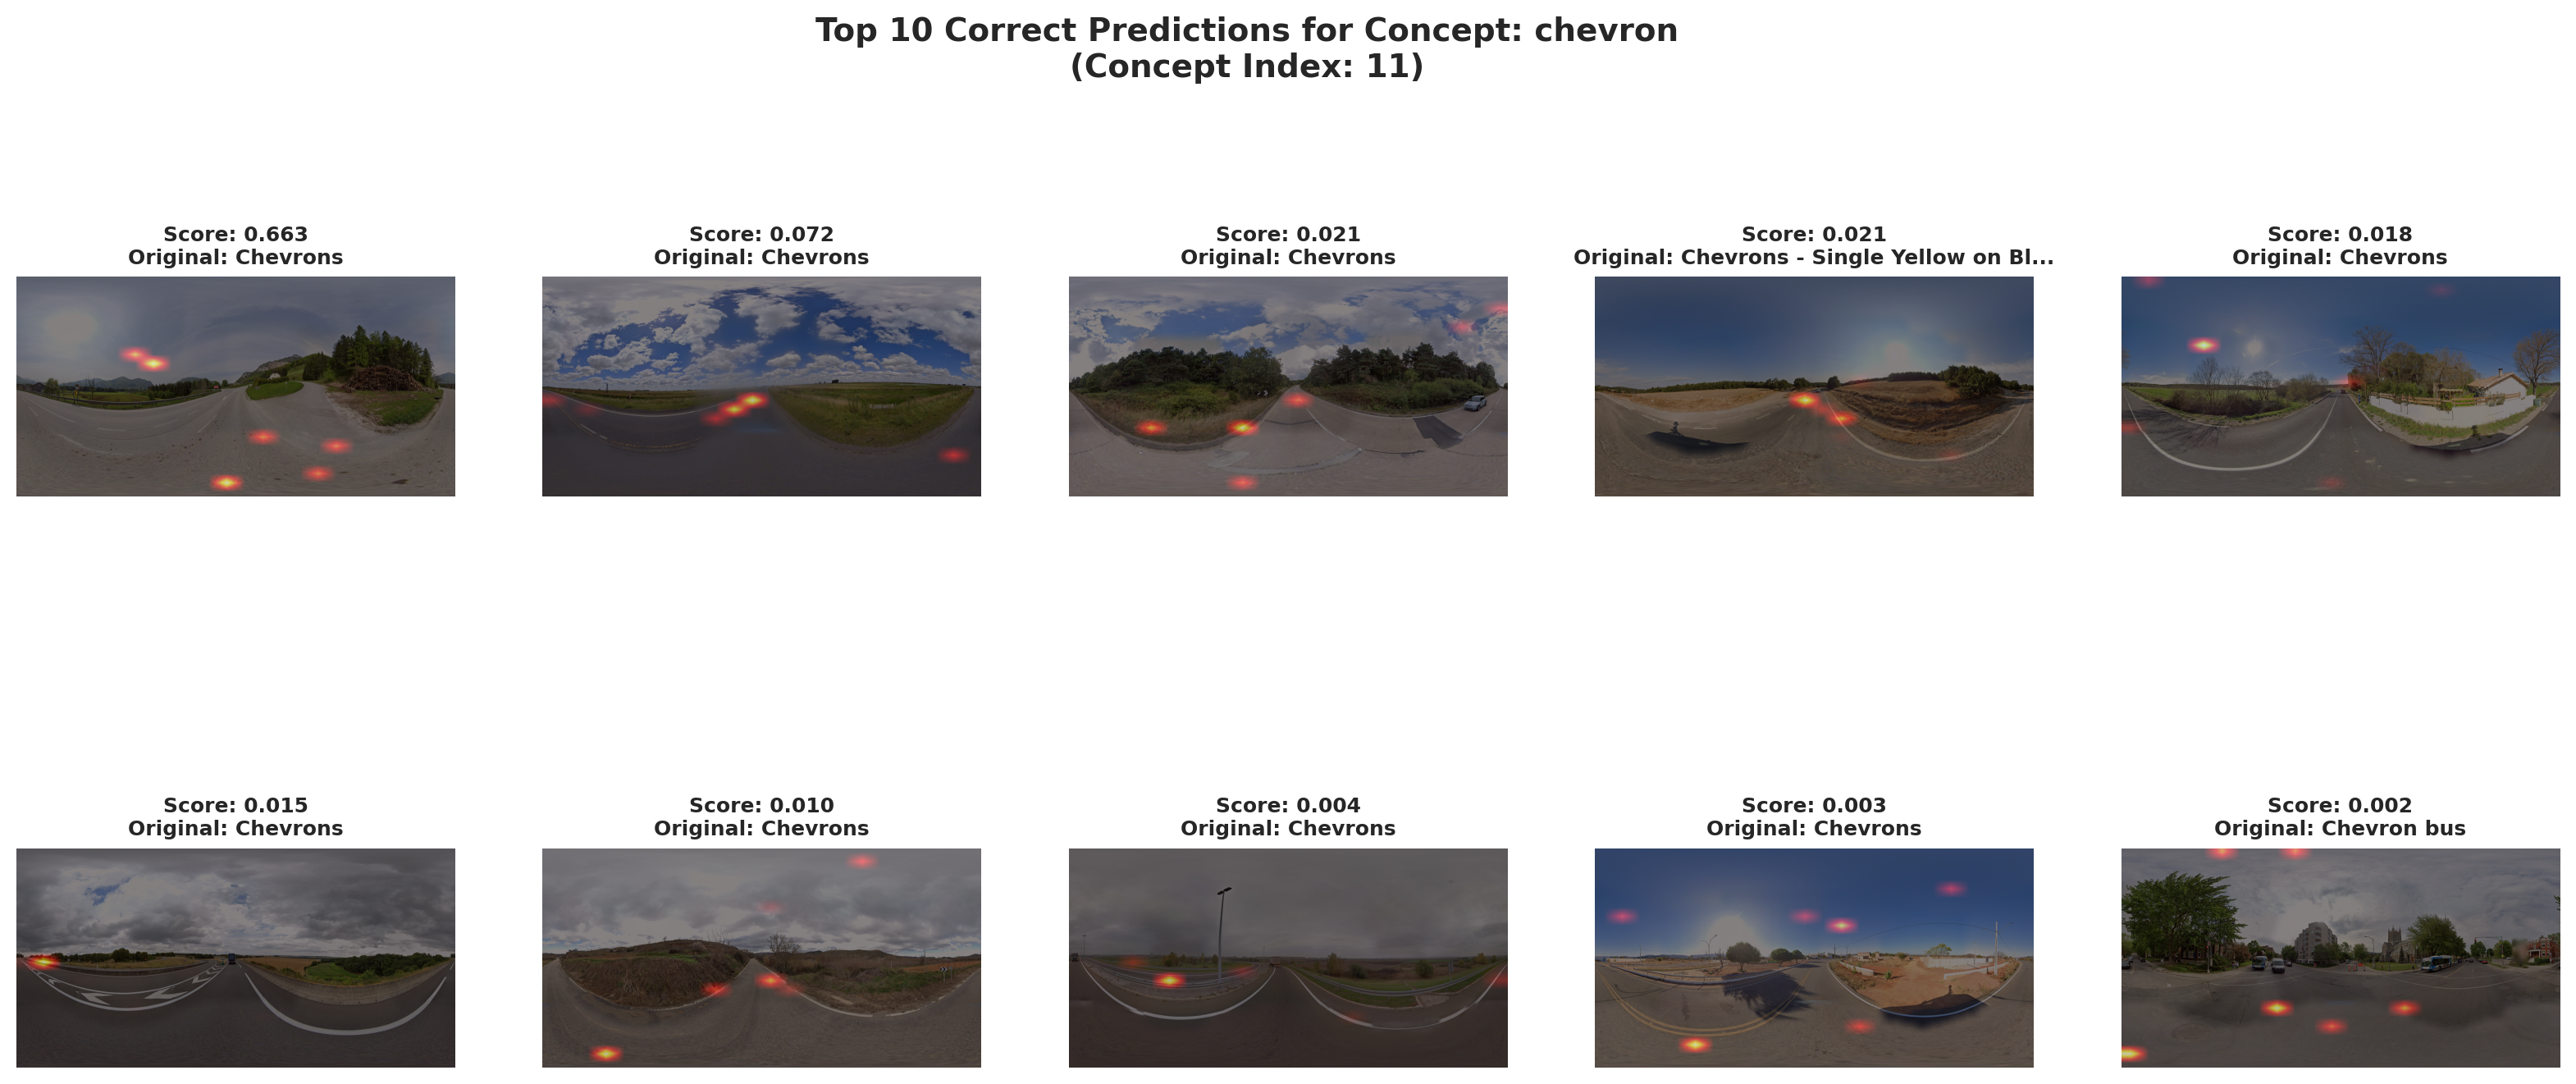
\includegraphics[width=\textwidth]{images/chevrons.png}
    \caption{Representative examples with ground-truth annotation for the \textit{chevron} concept, shown with patch-level evidence score overlays produced by the model. Images are ordered by decreasing concept activation score (reported above each image). While some examples exhibit localized activation on road markings consistent with chevrons, they do not overlay the actual chevrons in the image. Additionally, many cases select sky as the evidence, suggesting poor understanding of the concept. This highlights the challenge of detecting small, fine-grained structures such as chevrons at the StreetCLIP input resolution of $336 \times 336$ pixels, and is consistent with the low activation scores observed for this concept in the distribution analysis.}
    \label{fig:chevron_evidence}
\end{figure}


\begin{figure}[h]
\centering
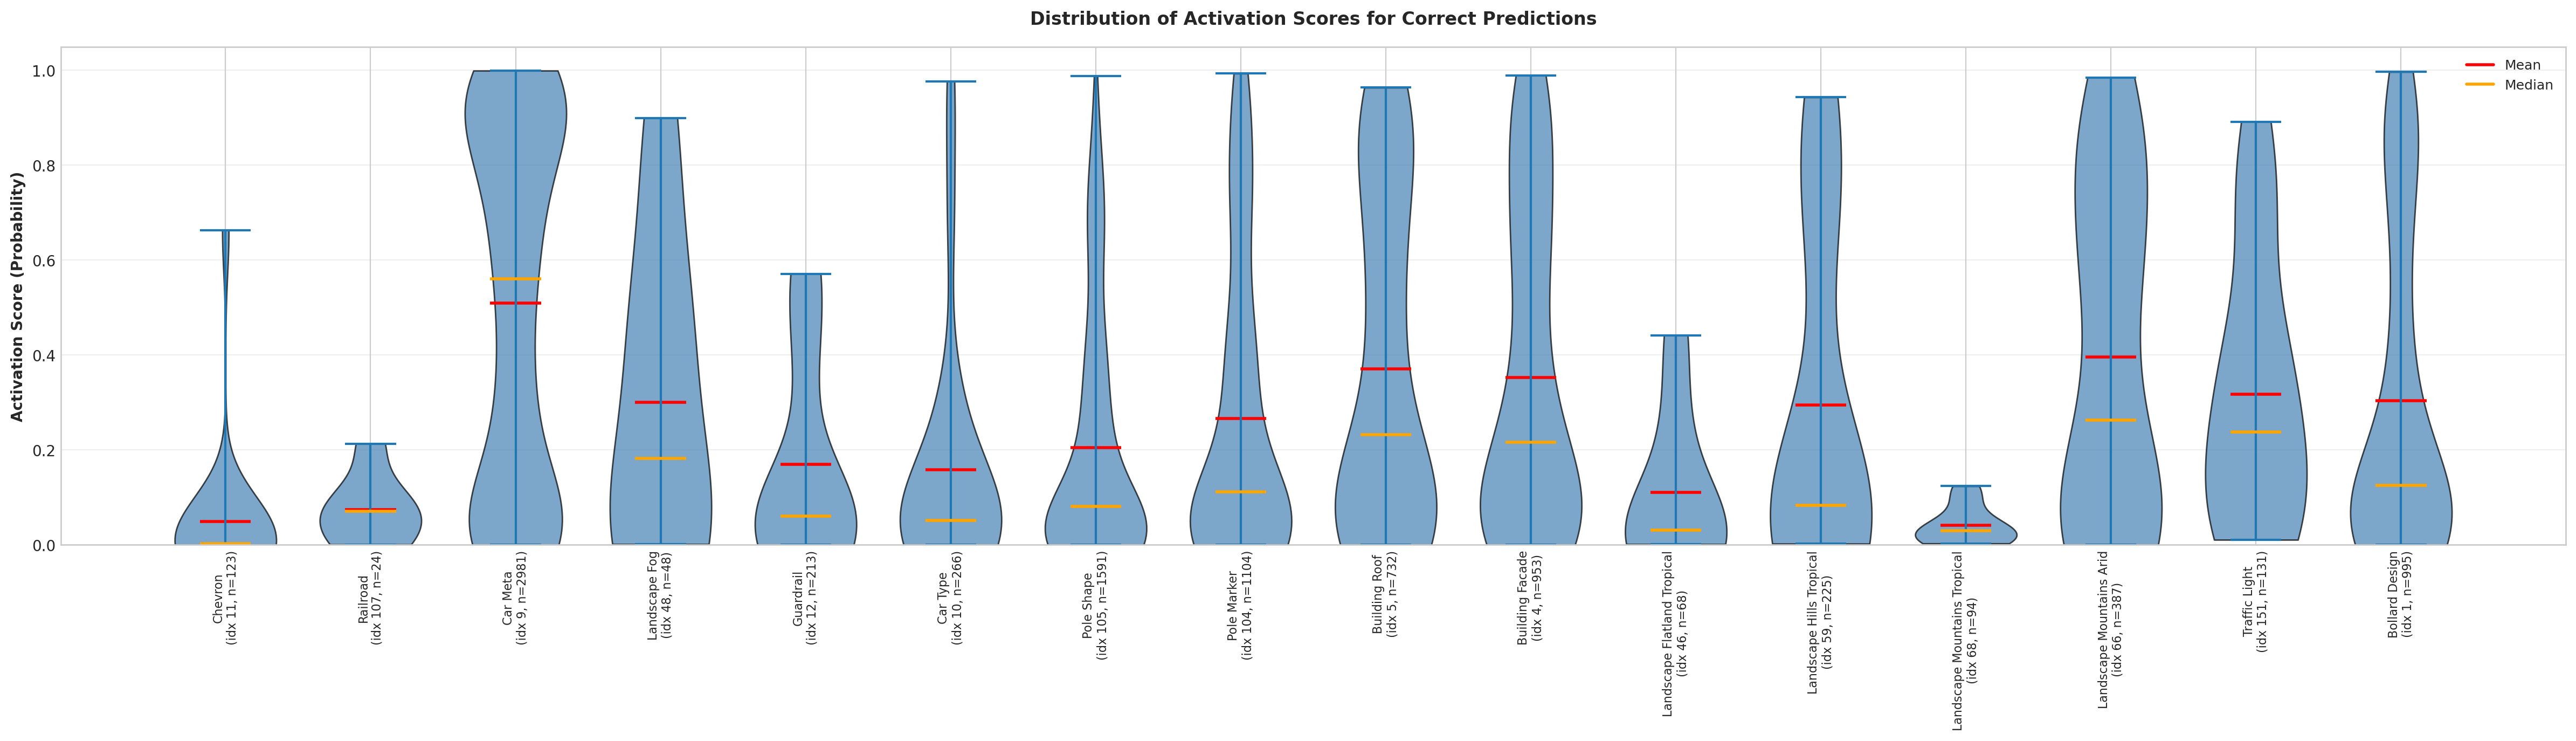
\includegraphics[width=0.9\textwidth]{images/activation_distributions.png}
\caption{Distribution of patch-level activation scores for selected concepts, evaluated on images where the corresponding concept is present. For each concept, we report the distribution of evidence scores across correctly predicted samples. The violin plots illustrate variability in activation strength across concepts, with mean (red) and median (orange) indicated. The results highlight systematic differences in activation behavior between fine-grained concepts (e.g., \textit{chevron}) and spatially extended concepts (e.g., landscape and building-related concepts), reflecting differences in visual scale and spatial coverage.}

\label{fig:evidence_distribution}
\end{figure}

In comparison, the \textit{bollard\_design} concept, which has a larger number of training examples, is detected more reliably in some cases (Fig \ref{fig:bollard_design_evidence}). However, its evidence score distributions indicate higher variability, and the corresponding evidence maps show that the concept is not consistently highlighted across all images where it is present. This suggests that increased training frequency alone does not guarantee stable patch-level activation.

\begin{figure}[t]
    \centering
    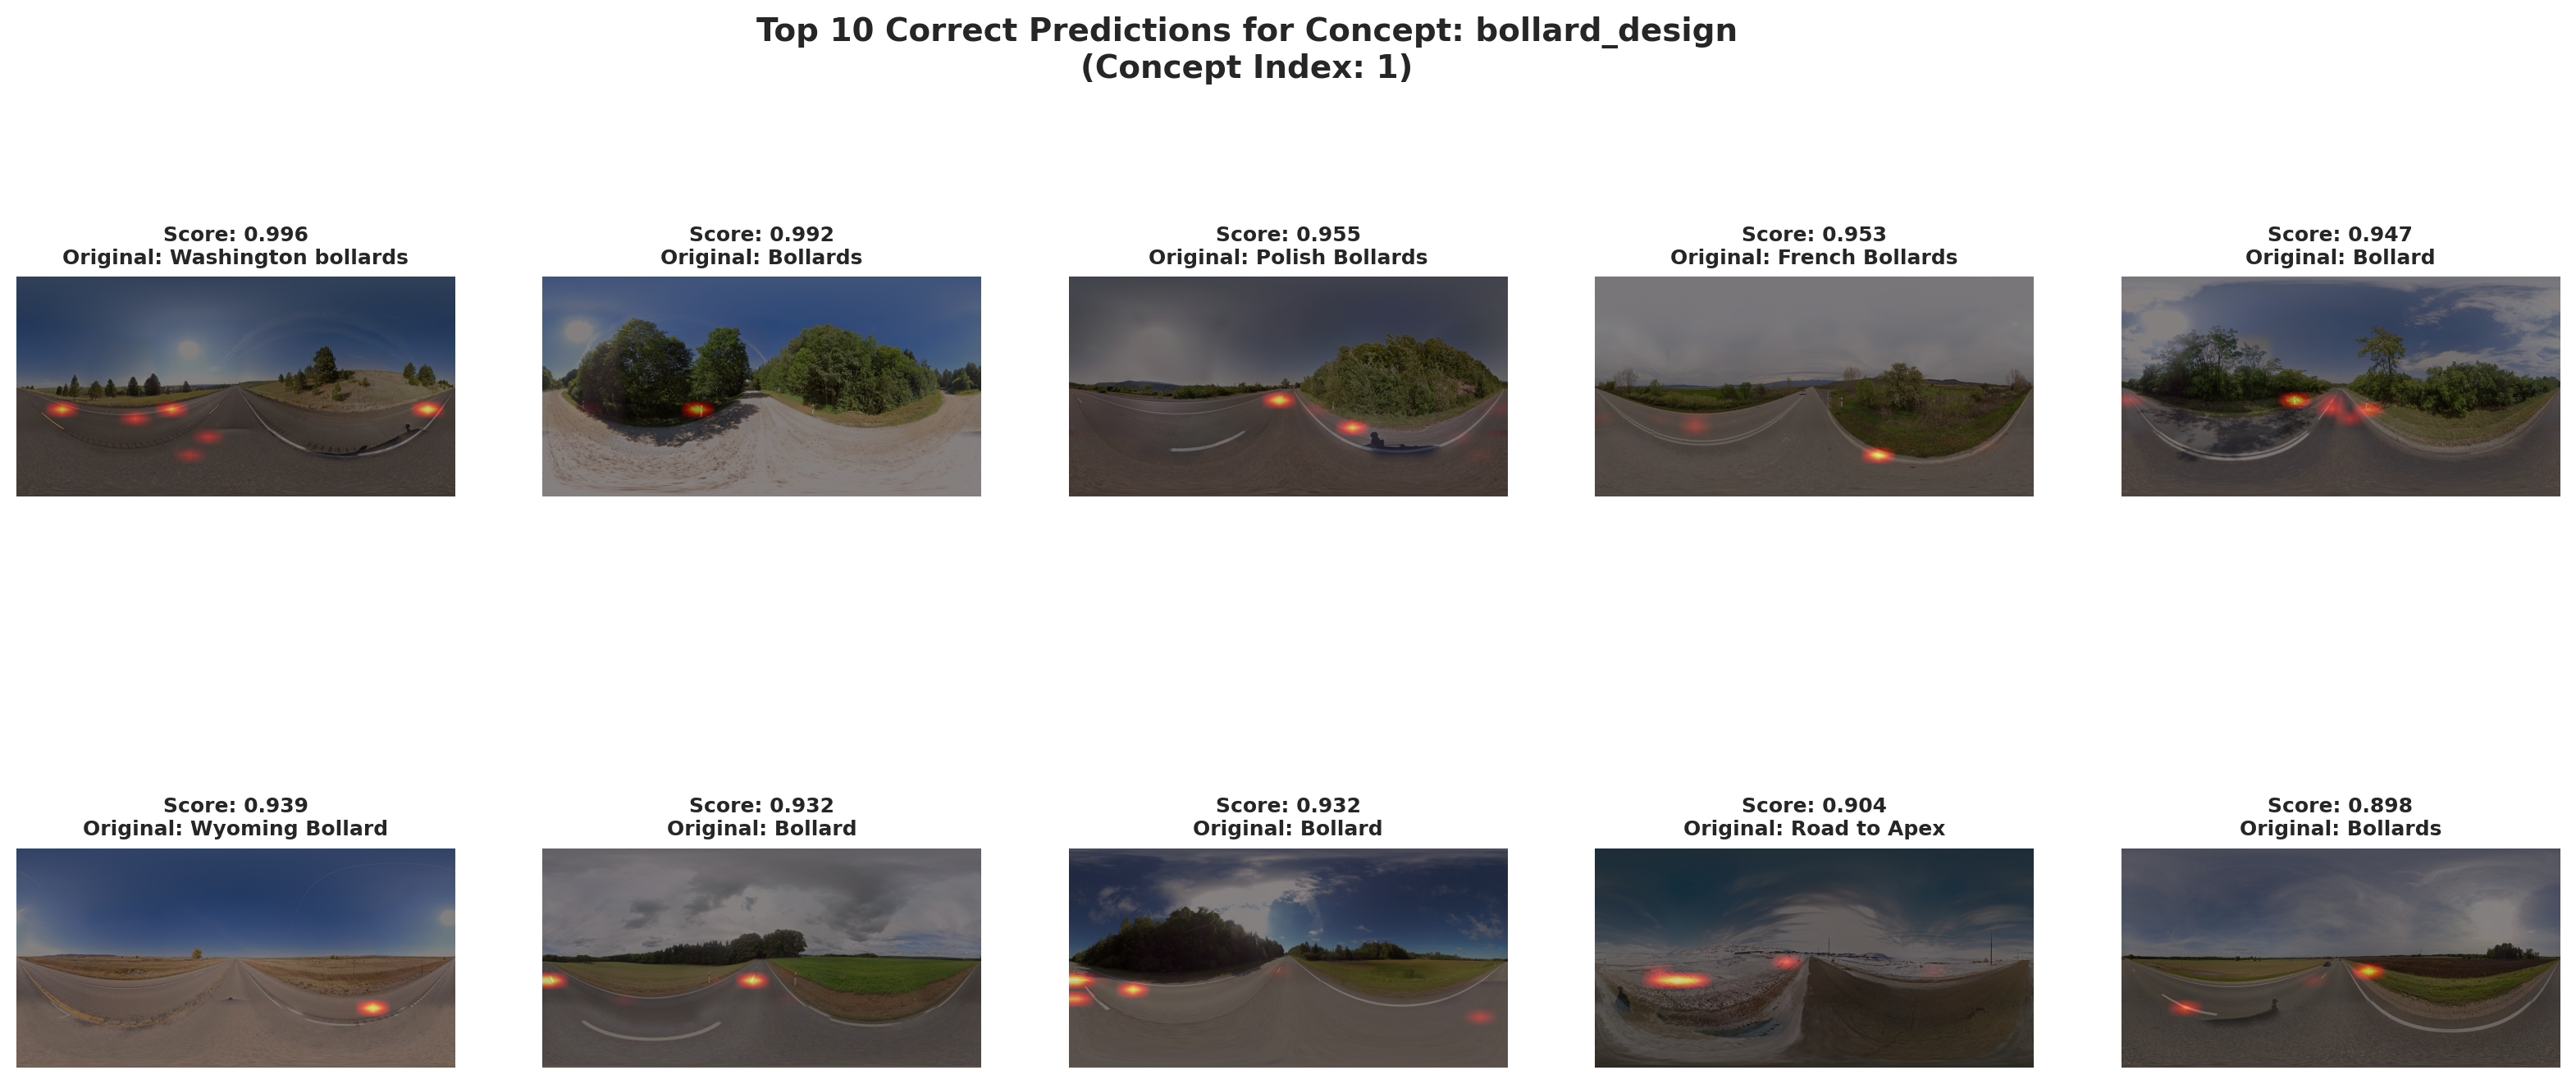
\includegraphics[width=\textwidth]{images/bollard.png}
    \caption{Representative examples with ground-truth annotation for the \textit{bollard\_design} concept, shown with patch-level evidence score overlays produced by the model. Images are ordered by decreasing concept activation score (reported above each image). In most cases, the evidence maps exhibit strong and spatially localized activation in the vicinity of roadside structures, though the model frequently focuses on the road region rather than exclusively on the bollard itself. This suggests that while the model reliably associates the concept with its typical visual context, fine-grained localization of the bollard object is not always achieved. These observations are consistent with the high but variable activation scores observed for this concept in the distribution analysis.}
    \label{fig:bollard_design_evidence}
\end{figure}



Conversely, concepts with fewer training examples but larger spatial footprint, such as \textit{landscape\_fog} (48 samples), show comparatively strong activation when present. This is further supported by their evidence maps (Fig \ref{fig:landscape_fog_evidence}), where fog regions are often highlighted across multiple patches. These observations indicate that activation strength is influenced not only by training frequency, but also by the visual extent and saliency of the concept in the image.

\begin{figure}[t]
    \centering
    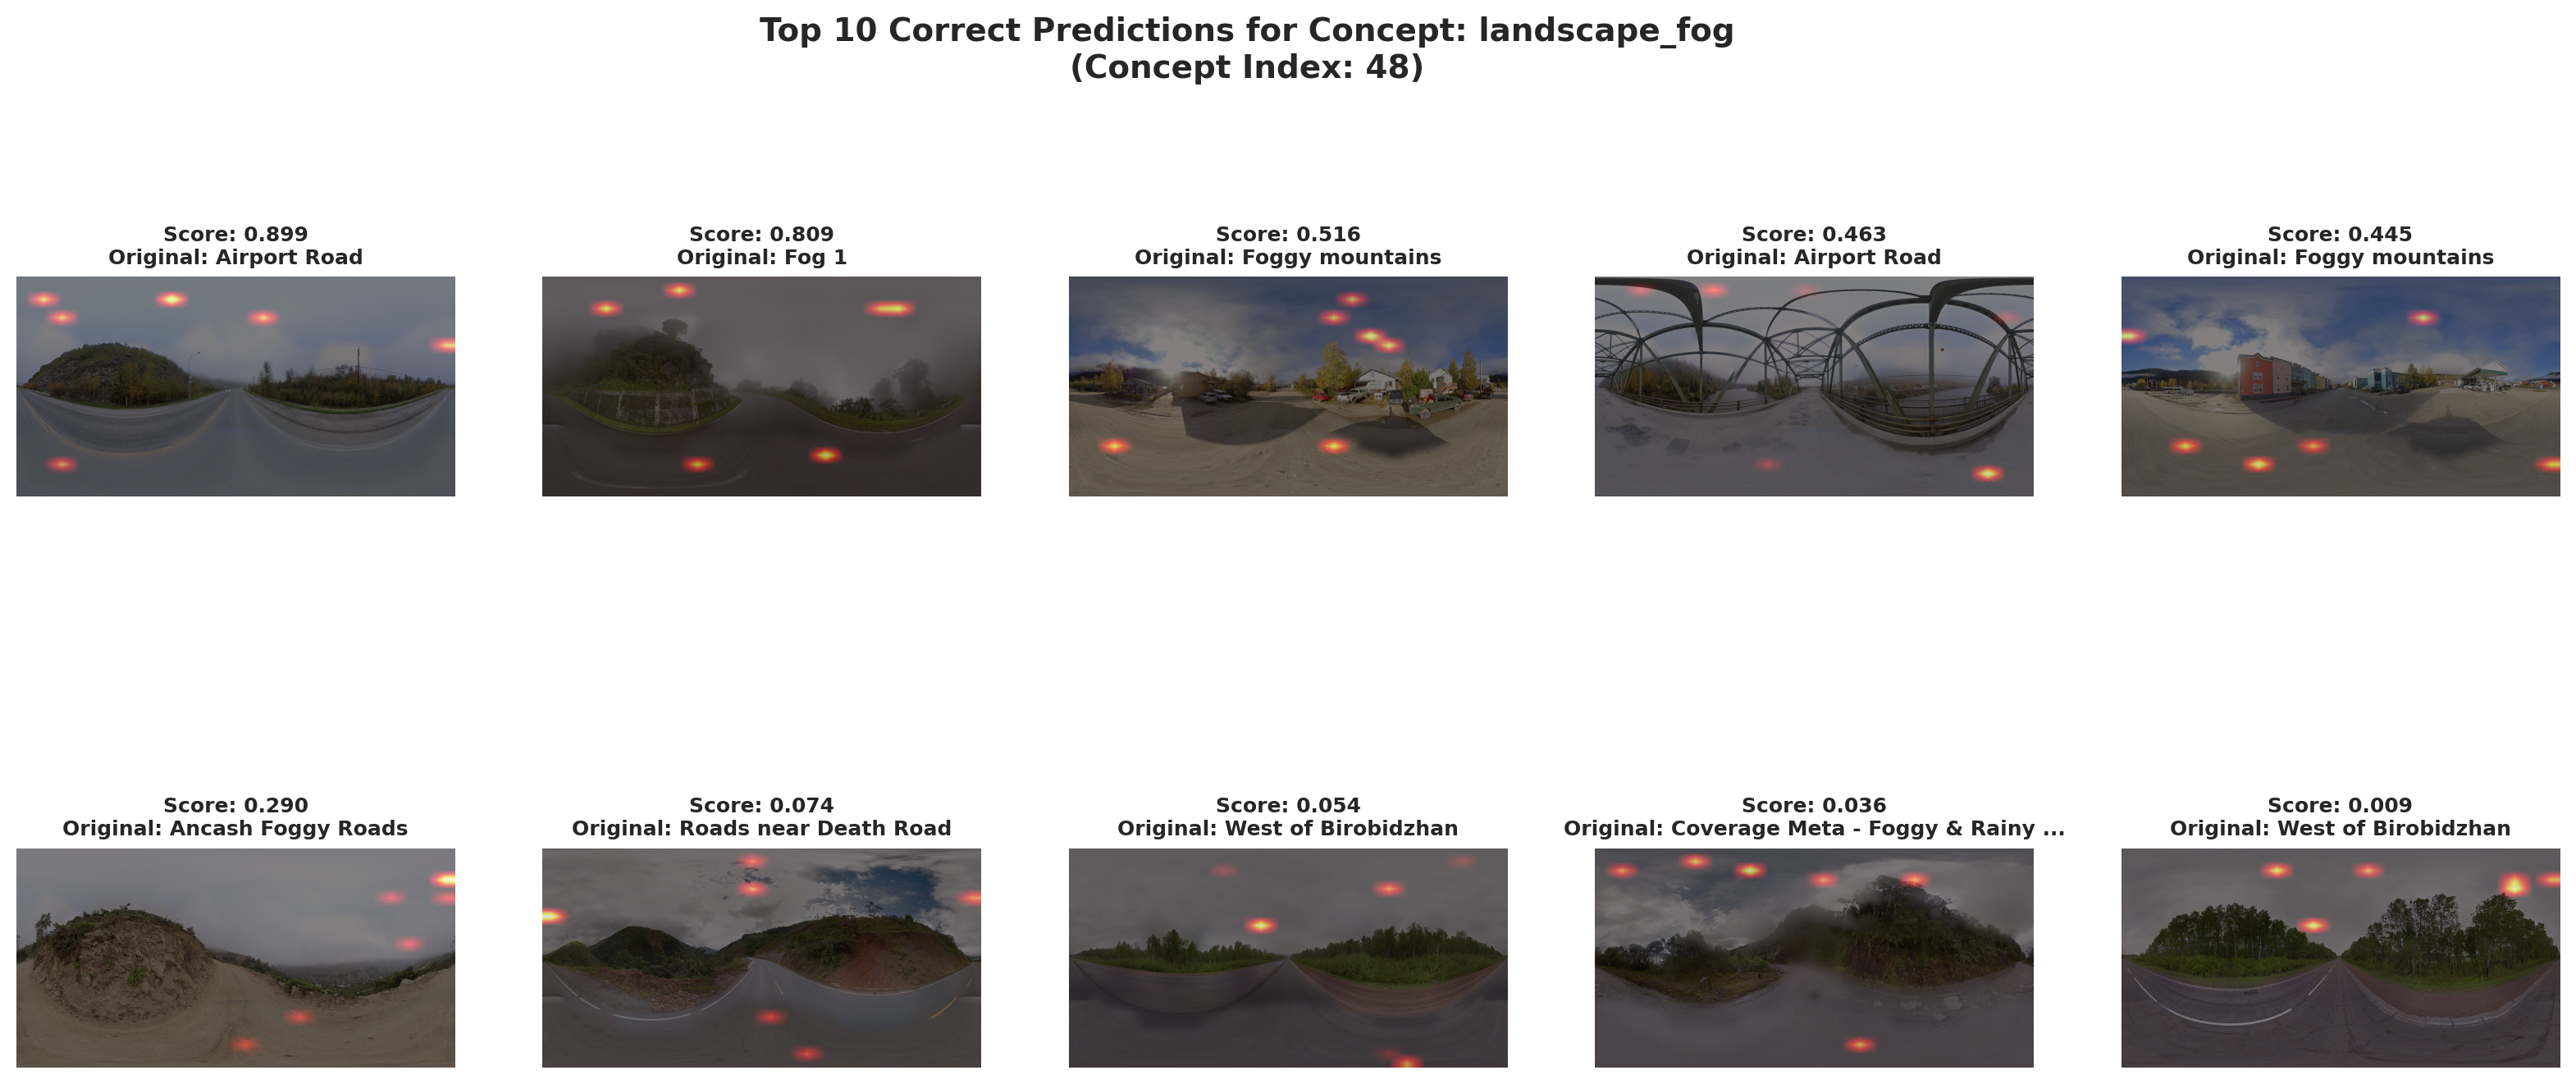
\includegraphics[width=\textwidth]{images/fog_makes_sense.png}
    \caption{Representative examples with ground-truth annotation for the \textit{landscape\_fog} concept, shown with patch-level evidence score overlays produced by the model. Images are ordered by decreasing concept activation score (reported above each image). The evidence maps tend to emphasize large, low-contrast regions consistent with fog (e.g., sky and distant background), rather than a single localized object, which is expected given the diffuse nature of the phenomenon. Despite the relatively small number of training examples for this concept, the model frequently produces clear activation when fog is visually present, consistent with the broader activation distribution observed for \textit{landscape\_fog} in Figure~\ref{fig:evidence_distribution}.}
    \label{fig:landscape_fog_evidence}
\end{figure}

The concepts \textit{building\_facade} and \textit{building\_roof} are closely related both semantically and visually, and frequently co-occur in the same images. Despite this similarity, the model exhibits distinct and concept-specific activation patterns for each. As shown in Figures~\ref{fig:building_facade_evidence} and~\ref{fig:building_roof_evidence}, the patch-level evidence maps highlight different regions of the image depending on the queried concept.
\begin{figure}[t]
    \centering
    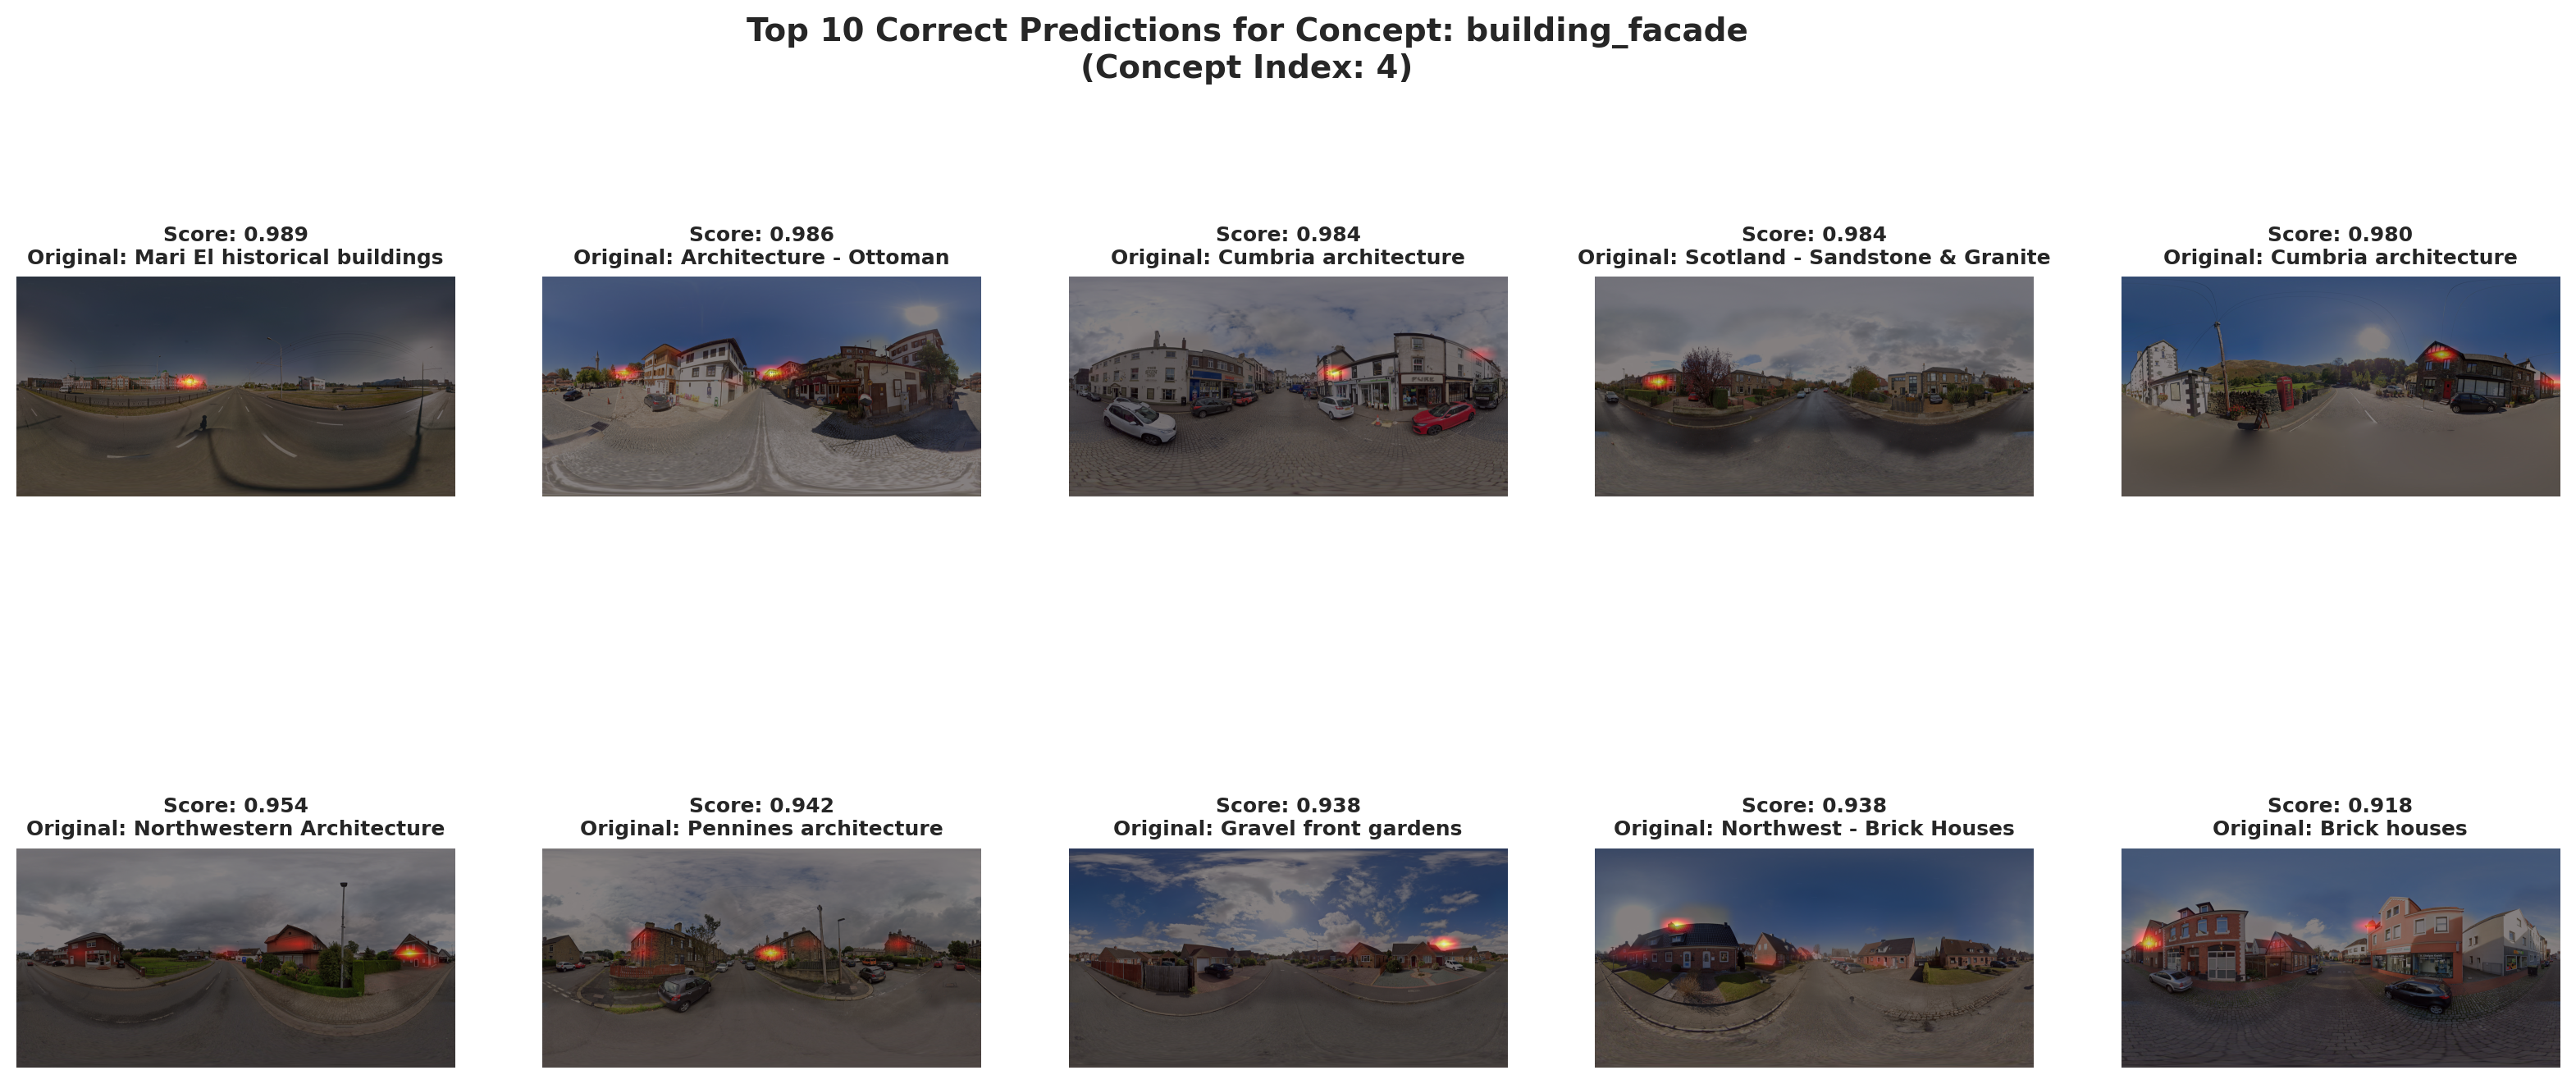
\includegraphics[width=\textwidth]{images/concept_0004_building_facade.png}
    \caption{Representative examples with ground-truth annotation for the \textit{building\_facade} concept, shown with patch-level evidence score overlays produced by the model. Images are ordered by decreasing concept activation score (reported above each image). The evidence maps predominantly highlight exterior surfaces of buildings, such as walls and facades facing the street, while largely excluding roof structures.}
    \label{fig:building_facade_evidence}
\end{figure}

For the \textit{building\_facade} concept, activations predominantly concentrate on vertical building surfaces, including walls, windows, and exterior materials facing the street. In contrast, the \textit{building\_roof} concept consistently emphasizes upper horizontal structures such as roof tiles, ridgelines, and thatched or elevated roofing elements. While both concepts may activate within the same scene, their evidence maps remain spatially distinct, indicating that the model does not simply rely on coarse building presence but instead differentiates between structural components.
\begin{figure}[t]
    \centering
    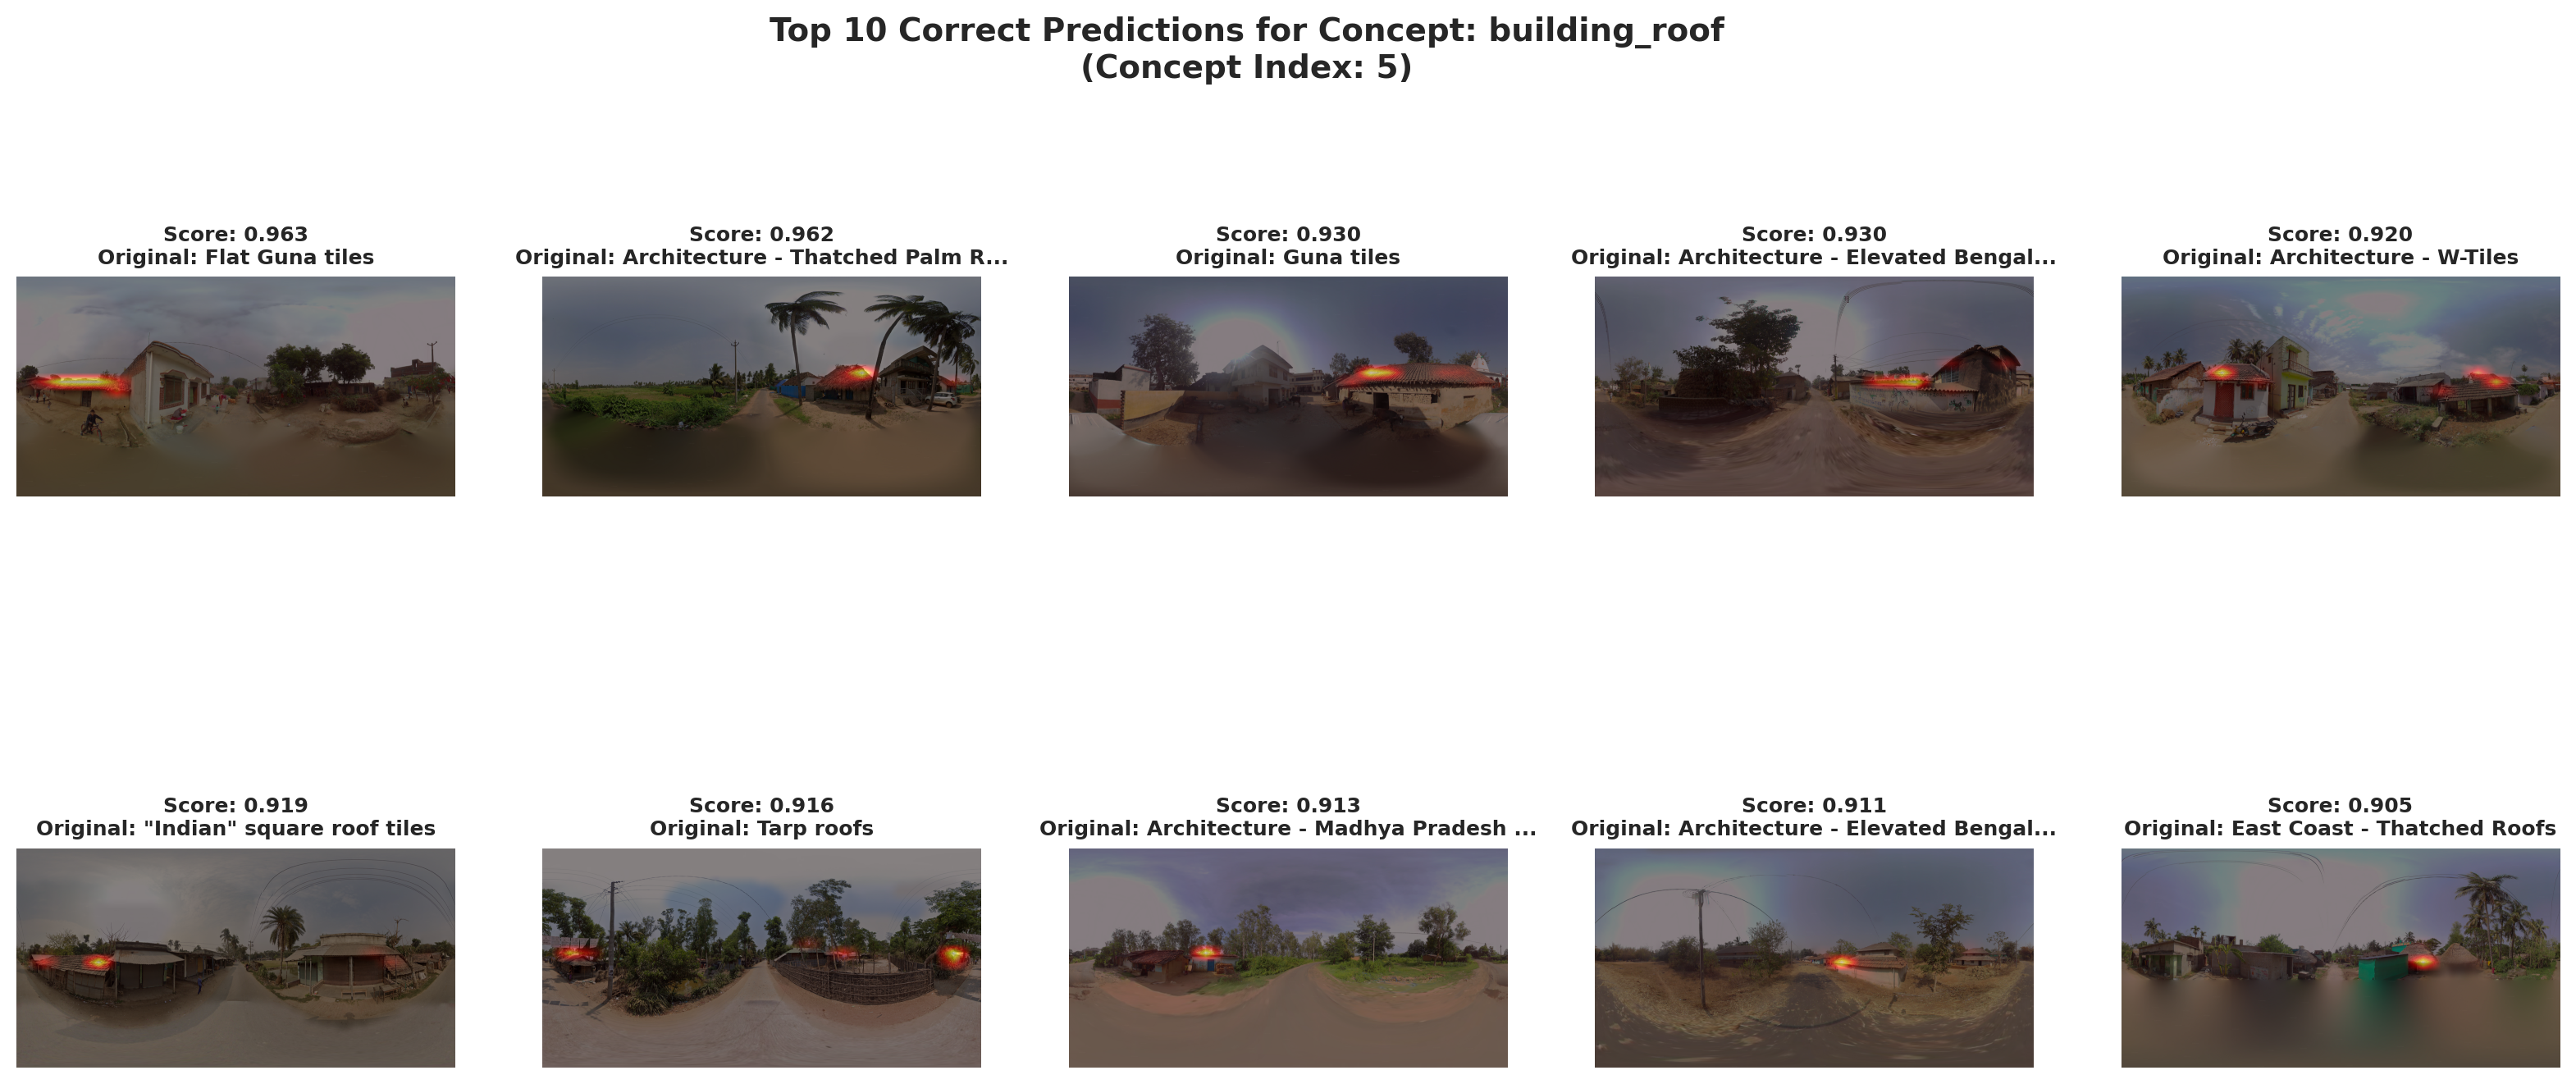
\includegraphics[width=\textwidth]{images/concept_0005_building_roof.png}
    \caption{Representative examples with ground-truth annotation for the \textit{building\_roof} concept, shown with patch-level evidence score overlays produced by the model. Images are ordered by decreasing concept activation score (reported above each image). In contrast to \textit{building\_facade}, the evidence maps concentrate on upper structural elements such as roof tiles, thatched roofs, and elevated roofing structures, with limited activation on building walls.}
    \label{fig:building_roof_evidence}
\end{figure}

This separation is particularly notable given the strong visual correlation between roofs and facades in many environments. The observed behavior suggests that the model learns concept-specific visual cues and assigns evidence at an appropriate spatial granularity, supporting interpretability even for semantically overlapping concepts.


\subsection{Geographic Analysis of Concept Effectiveness}



\section{Discussion}

\section{Conclusion}
\newpage
\bibliographystyle{plainnat}
\bibliography{references}

\newpage
\appendix







%%%%%%%%%%%%%%%%%%%%%%%%%%%%%%%%%%%%%%%%%%%%%%%%%%%%%%%%%%%%


\end{document}